\documentclass{article}
\title{CSC391 project2 report}
\author{Alex Zhang}
\date{Oct 2023}
\textwidth=16.00cm 
\textheight=22.00cm 
\topmargin=0.00cm
\oddsidemargin=0.00cm 
\evensidemargin=0.00cm 
\headheight=0cm 
\headsep=0.5cm
\textheight=610pt
\usepackage{graphicx}
\usepackage{multicol}

\graphicspath{ {./images/} }

\usepackage{latexsym,array,delarray,amsthm,amssymb,epsfig}
\usepackage{amsmath}
\usepackage{listings}
\lstset{
  basicstyle=\ttfamily,
  mathescape
}

\newcommand{\bmat}[1]{\begin{bmatrix} #1 \end{bmatrix}}
\newcommand{\mat}[1]{\mathbf{#1}}

\let\ds\displaystyle

\begin{document}
\maketitle
\section*{Part1}
\subsection*{Rotation}
In every case I tried to rotate the image to 270 degree clockwise.\\
For SIFT, I think the result shows that SIFT is rotation invariant after drawing the matches between two images.
The keypoints in the bed sheet and the human face can match with each other and the result shows that the accuracy is around 65\%.
The result matches the textbook's result.\\
\\
For FAST, in this case, the number of keypoints is already different.
After trying to create matching, I will say that FAST is not rotation invariant.
I must increase the threshold to make my code consider good matches.\\
\\
For Harris Corner Detection, there are only few matches.
I read from some online resources that Harris should be rotation invariant, so I check whether it will match without any rotation.
If there is no rotation, all keypoints are matched, but if there is a 270 rotation, really a few matched.
One probability is that there seems to be some identical corners like wood corners on both windows, it may confuse the detection.Second probability is that my hair seems to be smooth, it is hard to draw corners from Harris detection and the descriptor may also be confused.\\
\\
Using ORB seems to create many matches even if I rotate 270 degrees.
It has better accuracy than using SIFT.
One explanation for this is that when rotation degree is proportional to 90, ORB outperforms SIFT because the features for ORB usually stick to the center of image.
This will make feature matching easier because the position of features will always be vertical or horizontal.






\subsection*{Scale}
To test the scale invariant, I first shrink the image to 0.6 of the original.\\
For SIFT, I think it can still draw many matches with given keypoints, but compared to the original image, it still has many mismatches.
I consider SIFT as scale invariant because the accuracy is about 33\%.The result in the textbook is about 40\%.
One reason I think that SIFT didn't perform better when shrinking the image than expanding the image is that the number of keypoins decreases a lot when shrinking.
The percentage will decrease.\\
\\
I think FAST is scale invariant.
In my image, to say whether FAST is robust on scaling depends on the threshold.
In my case, there are lots of keypoints missing after I shank the image.
This will decrease the accuracy for finding matching features.
\\
For Harris corner detection, I think it also didn't do well if I try to shrink the image.
We can see that there are many mismatches if I only took part in matches.
Also, for the features that seem to be matched, my setting of threshold didn't count most of it because they are not close enough.
I can say Harris is not scale invariant.\\
\\
For ORB, I think it is scale invariant and it has even better results than SIFT.
One reason for this is that ORB has fewer features than SIFT and most of the features lie on that stripe pillow.
After shrinking the image, features on stripe pillows are still preserved which I think is the main reason for having better results than SIFT.



\subsection*{Low-light illumination}
I tried to make testing image to decrease the illumination.\\
For SIFT, the result indicates that SIFT is not really robust on low-light illumination.
Since there is no scaling or rotation, if we see a parallel line and the destination is the same, it is a good match.
Based on the matching feature, there are not so many parallel lines.\\
\\
For FAST, I saw many parallel lines.
I still think many features match with each other though there are some mismatches.
FAST should be robust to low-light illumination.
\\
For Harris, I think it is doing fine for low-light illumination.
There are many matches after I decrease the illumination.
I think the change for gradient on corners after decreasing light can still be detected for Harris.
So Harris corner detection should be robust for low-light illumination.\\
\\
For ORB, It is hard to say whether ORB is robust in low-light illumination or not.
It is true that there are some parallel lines, but there are also many intersections.
Based on my observation, it has similar performance with SIFT which is also what the textbook shows.
I think ORB can be robust for low-light illumination but not as good as FAST and Harris in this image.

\section*{Part2}
\subsection*{SIFT}
The following image is using SIFT as detector and descriptor.
\begin{figure}[ht!]
  \begin{center}
    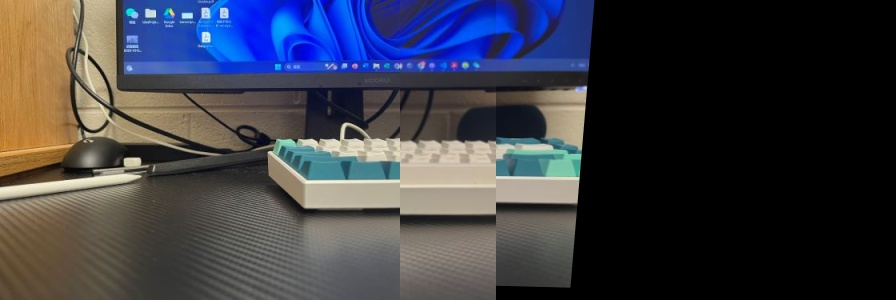
\includegraphics[scale=0.4]{SIFT-result.jpg}
    \caption[short]{SIFT}
    \label{fig:sift}
  \end{center} 
\end{figure}

\subsection*{BRISK}
the following image is using BRISK as detector and descriptor.
\begin{figure}[ht!]
  \begin{center}
    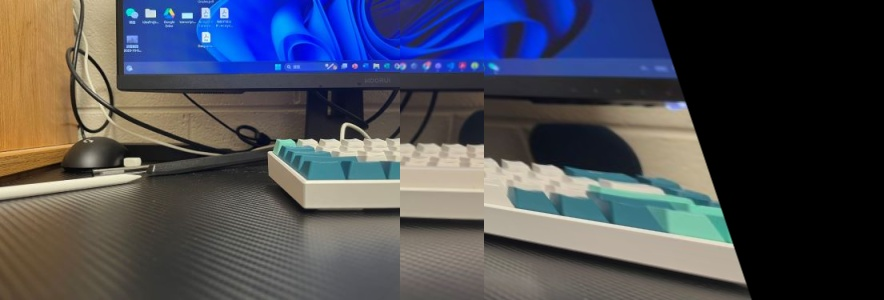
\includegraphics[scale=0.4]{BRISK-result.jpg}
    \caption[short]{BRISK}
    \label{fig:brisk}
  \end{center} 
\end{figure}
\subsection*{Harris}
The following image is using Harris corner as detector and SIFT as descriptor.
\begin{figure}[ht!]
  \begin{center}
    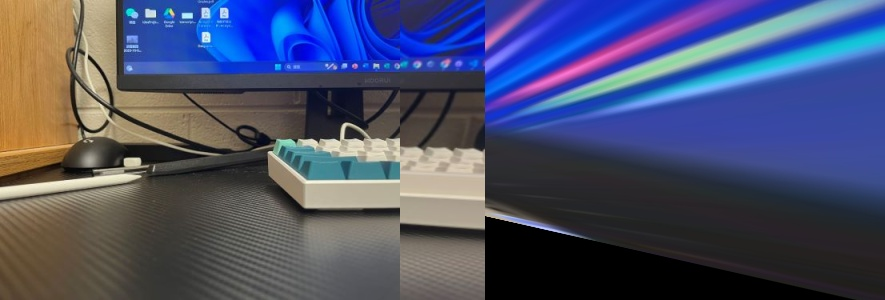
\includegraphics[scale=0.4]{Harris-result.jpg}
    \caption[short]{Harris}
    \label{fig:harris}
  \end{center} 
\end{figure}

\subsection*{ORB}
The following image is using ORB as detector asn descriptor.
\begin{figure}[ht!]
  \begin{center}
    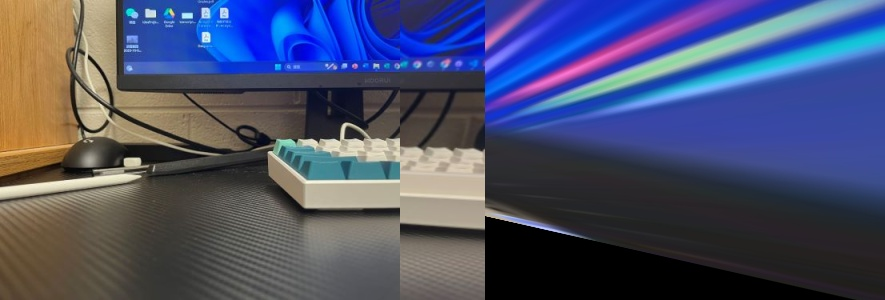
\includegraphics[scale=0.4]{ORB-result.jpg}
    \caption[short]{ORB}
    \label{fig:orb}
  \end{center} 
\end{figure}
\subsection*{Result}
From my observation, I think using Harris as a detector and SIFT as a descriptor has the best stitching.
SIFT as detector and descriptor is the following ones. ORB has the worst performance because I can hardly tell what object is in the last chunk.\\
\\
I'm surprised that Harris actually is the best among the four.
SIFT, ORB, and BRISK are well-developed feature matchers, and Harris is just a corner detector and it even used SIFT to find descriptors.
I thought the SIFT algorithm would at least be better than Harris.\\
\\
Also for ORB, I don't quite get it why it doesn't perform very well in this set of images.
I knew that OpenCV actually uses ORB in its stitcher class, indicating it should be kind of powerful.
One potential reason I think is that ORB needs more like parameters than the other three.
I even changed the threshold for good matches for ORB or it will not give me any output.
Another one is that ORB runs way faster than SIFT, probably this is also one reason why OpenCV chose it.\\
\\
To improve the quality, I think there are a few ways.
The first one is trying to combine different detectors and descriptors (Like Harris-SIFT). It may have better quality.
The second case is trying to rotate, scale, or increase the illumination for images before doing stitching.
SIFT didn't do well in low-light case, probably increasing the light will help SIFT better find matches.
Or analyze the image and extract some properties (like light, contrast), and apply the detector that has the best match in this case(FAST).
It is even possible to do multiple runs on different feature matchers.
Find the overlap between these matches and get the best-stitched image.

\section*{Part3}
One descriptor I learned about is BRIEF(Binary Robust Independent Elementary Features).
Basically, BRIEF stores feature descriptors in a binary encoding way. This can really reduce the storage requirement for keypoints descriptors.
It can also possibly increase the speed of generating descriptors.
I learned from opencv document that SIFT creates its keypoints descriptor by dividing sub-blocks from its neighborhood and creating a bin orientation histogram.
A total of 128 bin values are stored as a vector. This will take a lot of space. 
\\
BRIEF introduced pairwise intensity comparison based on image patches.
For example, in an image patch, first do smoothing by applying Gaussian kernel, and then choose n-pairs pixel (X, Y).
After choosing, define a test on the intensity of X and Y, if I(Y) is bigger than I(X), then its result is 1, else it will be 0.
The author of BRIEF's paper actually mentioned 5 different ways to choose n-pair, and they ended up choosing one isotropic Gaussian Distribution.
After conducting this method, they did some further tests and I observed that the speed for using BRIEF as a descriptor is much faster than using SIFT.
The computation time for the descriptor is about 30 times faster overall.
\\
For the recognition rate, BRIEF did really well compared to SIFT if we blur the image. 
Usually it has about 70\% of accuracy but SIFT only has around 50\% to 40\%.
However, we can further observe that BRIEF is not rotation invariant because once the rotation degree exceeds 30, the accuracy drops to around 0.
\\
In the paper, they use SURF as a detector and then BRIEF as a descriptor to do feature matching.
To further test how fast BRIEF can do in feature matching, I wrote some codes to measure the time doing SIFT for detector and descriptor, and the time for SIFT as detector and BRIEF as descriptor.
It turns out that for a really small image, BRIEF always runs faster than SIFT (0.05 second compared to 0.09 second). We can even increase the time by replacing FAST as a detector instead of using SIFT(0.02 seconds this time).\\
\\
For the application of feature detection, I asked this question to chatGPT, and I found one application for feature detection is medical imaging.
There should be some really complicated algorithm for feature matching that identifies special structures like blood vessels and tumors.
People need to have an algorithm that is scale invariant, rotation invariant, and light invariant because some anatomical landmarks have different sizes, and are in different positions which requires an accurate algorithm to identify.
Usually, this involves many usage of different detection methods and deep learning is frequently used.


\end{document}